\chapter{NoSQL Injection Mitigation}
Within this section, a mitigation approach for injection attack against non-relational databases is presented. Based on the previous attack analysis and classification, a new prevention concept is elaborated addressing the major design problems. Further, a feasible way for the implementation of the presented mitigation technique is outlined and empirically evaluated.

\section{Conception}
In order to create an mitigation concept for NoSQL injection, the exposed design problems have to be considered. The last chapter concludes four major issues, that lead to injection vulnerabilities of non-relational databases. Since error-prone string escaping is a well known and actually problem, the fourth class is not focused. The main issue brought along with non-relational databases is object structure defined semantic. This feature gives a raise to attacks based on error-prone type and structure escaping as well as diverging parameter handling. As exposed by the found attacks, problems of this kind are spread across all investigated databases and application layers. The third class of attacks is bases on shared storage scopes and is only present for CouchDB. This issue can be solved by strict data separation. Therefore, the main goal for attack mitigation is the prevention of type and object structure injection. This addresses two-thirds of the found injection attacks and represents a problem not adequately solved yet. \\

The first idea regarding the mitigation of type and object structure based injection attacks, may be simple type casting of parameters. Although, this strict method would prevent most attacks, it has major drawbacks. On the one hand, the required type casting is highly dependent on the use case and performed query. With this technique, developers are responsible for attack mitigation by applying suitable type castings for each query parameter. This resembles the idea of manual parameter escaping for SQL statements, which was not reliably applied by developers. A vital argument against type casting, is the flexibility required by many applications. Listing \ref{lst:ExampleFindQueryStringID} and \ref{lst:ExampleFindQuerySpecialID} exemplify a use case, that employs two different types of identifiers. \\

\begin{minipage}{.97\textwidth}
\begin{minipage}[t]{.49\textwidth}
\begin{lstlisting}[escapechar=!, caption={Example for find query with a string identifier}, label={lst:ExampleFindQueryStringID}]
db.find({
  "_id": !\textbf{"56767834"}!

});
\end{lstlisting}
\end{minipage}
\hfill
\begin{minipage}[t]{.49\textwidth}
\begin{lstlisting}[escapechar=!, caption={Example for find query with a special object identifier}, label={lst:ExampleFindQuerySpecialID}]
db.find({
  "_id": {
    !\textbf{"\$oid": "54651022bffebc03098b4567"}!
});
\end{lstlisting}
\end{minipage}
\end{minipage}

The given queries work on a database, that contains documents with varying identifier formats. Some documents use a string based identifier, others employ an object-based identifier. The latter type is used in order to indicate a special format of the stored identifier string. Such differences of data types are typical for non-relational databases, due to their ability to handle unstructured data. The highlighted parts of the code have to be under user control, to allow generic querying of both identifier types. In contrast to the given scenario, such querying becomes arbitrary complex depending on the number of different property types within the database. Type casting for the highlighted parameter can therefore not be applied. In summary, some use cases require structural control of user-provided query parameters. \\

So why not apply type casting of parameters where possible and otherwise grant full flexibility? Regarding the example given with listing \ref{lst:ExampleFindQueryStringID} and \ref{lst:ExampleFindQuerySpecialID}, query selector injection is still an issue. Therefore, the full flexibility has to be restricted a bit. At this point, the mitigation approach of this thesis applies. In order to grant a certain degree of flexibility, but still prevent injection, allowed parameter structures have to be defined for each query. Based on the requirements, this thesis suggest a pattern-based control mechanism for query parameterization. The patterns define a range of allowed query structures and the all others are blocked. This approach applies directly at the connection between application and database layer, within the database driver. Therefore, each input for the query can be reliably filtered without any danger of subsequent manipulation. \\

The presented approach still requires manual pattern definition for each query, but in contrast to type casting at least allows some kind of flexibility for query parameters. This idea can be taken a step further to bring another important advantage. The creation of the applied security patterns can be automatized. Basically, the idea is to learn the patterns in a secure execution environment of the application. In a second step, the application goes live and the pattern validation is activated. This can be seen as a learning and an execution phase. Software tests are normally present for each application and constitute a great means to build the security patterns based on trusted inputs. By providing such a framework, a solution independent from the underlying technology stack, concrete security patterns and implementation details is given. This approach provides the needed flexibility, does not require high engineering efforts and provides sufficient protection from the found injection attacks.

\section{Implementation}
The previously described mitigation technique for NoSQL injection attacks has to be transformed into practice. For the exemplary implementation outlined within this section, the most prevalent technology stack was selected. According to the statistics shown in chapter \ref{cha:intro_to_nosql_injection}, MongoDB and NodeJS represent the most widespread technologies relevant in scope of this thesis. As exposed by the initial investigation, this combination of application and database layer reveals severe weak spots for injection attacks. Therefore, an exemplary implementation of the presented mitigation technique is given for NodeJS applications running on MongoDB. \\ 

To stop object structure and type injections, all affected query parameters have to be sanitized. The most reliable way to accomplish this sanitizing, is an integration of the mitigation technique directly into the database driver. In avoidance of writing an entirely new database driver, the existing MongoDb driver for NodeJS is used and wrapped with an additional layer. The rough architecture and functioning of the implementation is visualized by figure \ref{fig:architecture_secure_driver}. \\

\begin{figure}[h]
\centering
  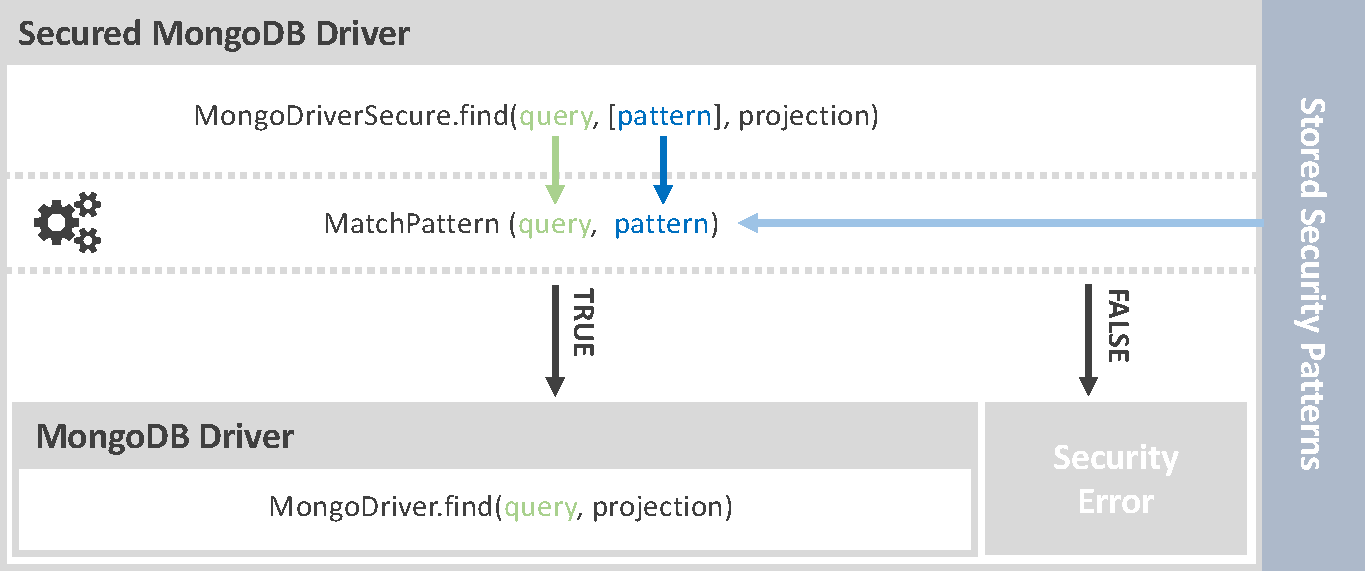
\includegraphics[width=1\linewidth]{Images/secure_driver}
  \caption{Architecture for the implementation of the NoSQL injection mitigation concept}
  \label{fig:architecture_secure_driver}
\end{figure}

Basically, the secured driver extends the former interface with optional \emph{pattern} arguments. These follow can be passed after the sensitive argument and define the allowed data types and structures. The shown example extends the find function with an optional security pattern for the \emph{query} argument. When no security pattern is provided by the arguments, the driver can alternatively draw on stored ones. These stored security patterns can be created automatically within a secure execution environment. In order to prevent injection, the extended driver matches the given security pattern with the passed argument. When both are compatible, all arguments except of the security patterns are forwarded to the normal MongoDB driver. Otherwise, a security error is thrown, that indicates a potential injection attack. In case no security pattern is provided, the query parameter are passed without further control to the wrapped driver. This behavior enables a drop-in replacement of the secured driver without breaking any application. Similar to this implementation, drivers for other databases and application layers can be wrapped. \\

At this point, the employed security pattern structure has to be defined. There exist various possible ways to implement the patterns for the presented mitigation approach. This thesis proposes a JSON-based format for straightforward handling across all feasible application layers. Listing \ref{lst:http_request_example} shows the grammar of the security patterns used for the outlined implementation. \\

\begin{lstlisting}[escapechar=!, caption={Proposed security pattern grammar for the the injection mitigation mechanism}, label={lst:http_request_example}]
<SecurityPattern> ::= {'_security_pattern': <Option> };
<Options> ::= <Option> | <Option>, <Options>;
!\textbf{<Option> ::= [<Values>]}!;
<Value> ::= <Array> | <Object> | <Type>;
<Array> ::= [] | [!\textbf{<Options>}!];
<Object> ::= {} | {<Properties>};
<Values> ::= <Value> | <Value>, <Values>;
<Properties> ::= <Property> | <Property>, <Properties>;
<Property> ::= <Key> : !\textbf{<Option>}!;
<Type> ::= "String" | "Number";
<Key> ::= *Arbitrary String*;
\end{lstlisting}

The given grammar for the security patterns resembles the one of JSON. On the top level, the \emph{\_security\_pattern} property is fixed, to be able to distinguish normal and pattern arguments. Furthermore, each value of objects and arrays is replaced by an option array as highlighted. This allows the declaration of multiple allowed types and structures and ensures the required flexibility. The options array in turn contains other structures or type definitions. In order to keep the grammar neat, the last rule for arbitrary key strings is shortened. Strings and numbers are indicated with the according string, arrays an objects are represented by the actual JSON elements. Since this may be hard to imagine, a practical example is given within listing \ref{lst:http_request_example}. \\

\begin{lstlisting}[escapechar=!, caption={Security pattern allowing string-based and object-based identifiers as a query parameter}, label={lst:http_request_example}]
{"_security_pattern_": [{
  "_id": ["String", {"$oid": ["String"]}]
}]}
\end{lstlisting}

This security pattern is tailored to the motivational example given by listing \ref{lst:ExampleFindQueryStringID} and \ref{lst:ExampleFindQuerySpecialID} in the previous section. Two alternatives are listed for the \emph{\_id} property. Either a string value can be passed or an object containing a string-based property with the key \emph{\$oid}. The pattern can be passed as an additional parameter to the secured MongoDB driver or created with the help of exemplary queries. Thereby, the advantage of the options array for automatic pattern learning becomes clear. For each observed query that is not covered by the pattern, an additional option can be appended to the array. 


\section{Evaluation}
\label{sec:evaluation}
Within this section, the designed mitigation technique for NoSQL injection is evaluated by means of the outlined implementation. First, the applied methodology is explained and afterwards, the evaluation results regarding compatibility and security are summarized.

\subsection{Methodology}
In scope of this evaluation, two major aspects of the injection mitigation technique have to be considered. The first one is the compatibility of the implemented solution with existing applications. A mitigation approach, that requires high engineering efforts and code changes to be compatible, would not be viable in practice. The other aspect is the provided security form injection attacks against the underlying database. This security aspect has to be evaluated with regard to the addressed attack classes. \\

In order to give an empirical evaluation, a group of open source applications is selected. These applications have to be built with NodeJS and MongoDB, to allow the integration of the implemented secure driver. To enable the required driver integration, the code of the selected applications have to be openly accessible. Based on this criteria, the following widespread projects were selected for the further evaluation.

\begin{description}
\item [Agora] This project is developed by the German Softwerkskammer and builds the central platform for their communities. [https://github.com/softwerkskammer/Agora]
\item [Apostrophe 2] With the goal of an design-driven and flexible content management system, Apostrophe bets on NodeJS and MongoDb for its most current version. [http://apostrophecms.org/]
\item [Habitica] This project set its objective, to create a productivity enhancing and habit building application with the help of an integrated gamification concept. [https://habitica.com] 
\item [NodeBB]  The goal of this platform is to deliver a powerful and mobile-ready forum software for the modern web. [https://github.com/NodeBB/NodeBB]
\item [Pencilblue] This application represents an open source content management system for business class use cases. [https://pencilblue.org/]
\end{description}

Next to the listed projects, also the original MongoDB driver for NodeJS is considered for the evaluation. The general approach is, to utilize the tests available for each of the applications. In a first step, these test are executed and the number of passed ones is measured. Then, the existing MongoDB driver is replaced with the secured one. The same tests are run again with the changed setup and the number of passed ones is again measured. Thus, the measured ratios of passed test can be compared for each application. With regard to the security aspect, it represents a problem to find an appropriate measurement. The mitigation of real world vulnerabilities would be an feasible approach, but these are not available in scope of this work. Therefore, the guarantees given by the new driver implementation and the coverage of attack classes are evaluated.

\subsection{Compatibility}
The measurement of the passed tests with the normal as well as the secured driver lead to the results, presented within table \ref{tab:compatbility_eva_overview}. 

\begin{table}[h]
  \sffamily
  \centering 
  \begin{tabular}{llcc}
  \multirow{2}{*}{\textbf{Application}} & \multirow{2}{*}{\textbf{Type}} & \multicolumn{2}{c}{\textbf{Passed Test Rate}} \\ 
    & & \textbf{Normal Driver} & \textbf{Secured Driver}  \\ \hline
  MongoDB driver & Database Driver & 100\% & 100\% \\
  Agora & Groupware Platform & 100\% & 100\% \\
  Apostrophe 2 & Content Management System & 100\% & 100\% \\
  Habitica & Habit building program & 100\% & 100\% \\
  NodeBB & Forum Software & 100\% & 100\% \\
  Pencilblue & Content Management System & 100\% & 100\% \\ \hline
  \end{tabular}
  \caption{Rate of passed tested with normal and secured MongoDB driver}
  \label{tab:compatbility_eva_overview}
\end{table}

% without learned pattern, since this is a extra topic. Manuall securing possible without breaking the existing applicaiton
% the normal driver can therefore replaced by secured driver allowing optional pattern arugments

\subsection{Security}
The security provided by the mitigation technique integrated into the database driver is highly dependent on the underlying security patterns. It has to be emphasized, that the implemented driver does only provide protection, when security patterns are defined. This can happen through the additional query parameters or the approach of automatic pattern learning. Even when the security patterns are provided, the reliability of the mitigation approach still depends on the quality of the patterns. In case of pattern learning, the quality is influenced by the trusted environment. When during the learning phase not each possible query parameter format is covered, the false-positive rate of the execution phase will increase. On the assumption of perfect security patterns, all injection classes depending on object structure and type manipulation can be reliably prevented. Injection classes based on error-prone string escaping or shared data storage are not covered by the mitigation approach.